\chapter{Analysis of the MICEGUT dataset}
\section{Dataset Description}
\textcolor{red}{to be completed}
\begin{figure}[H]
\centering
\fcolorbox{black}{white}{
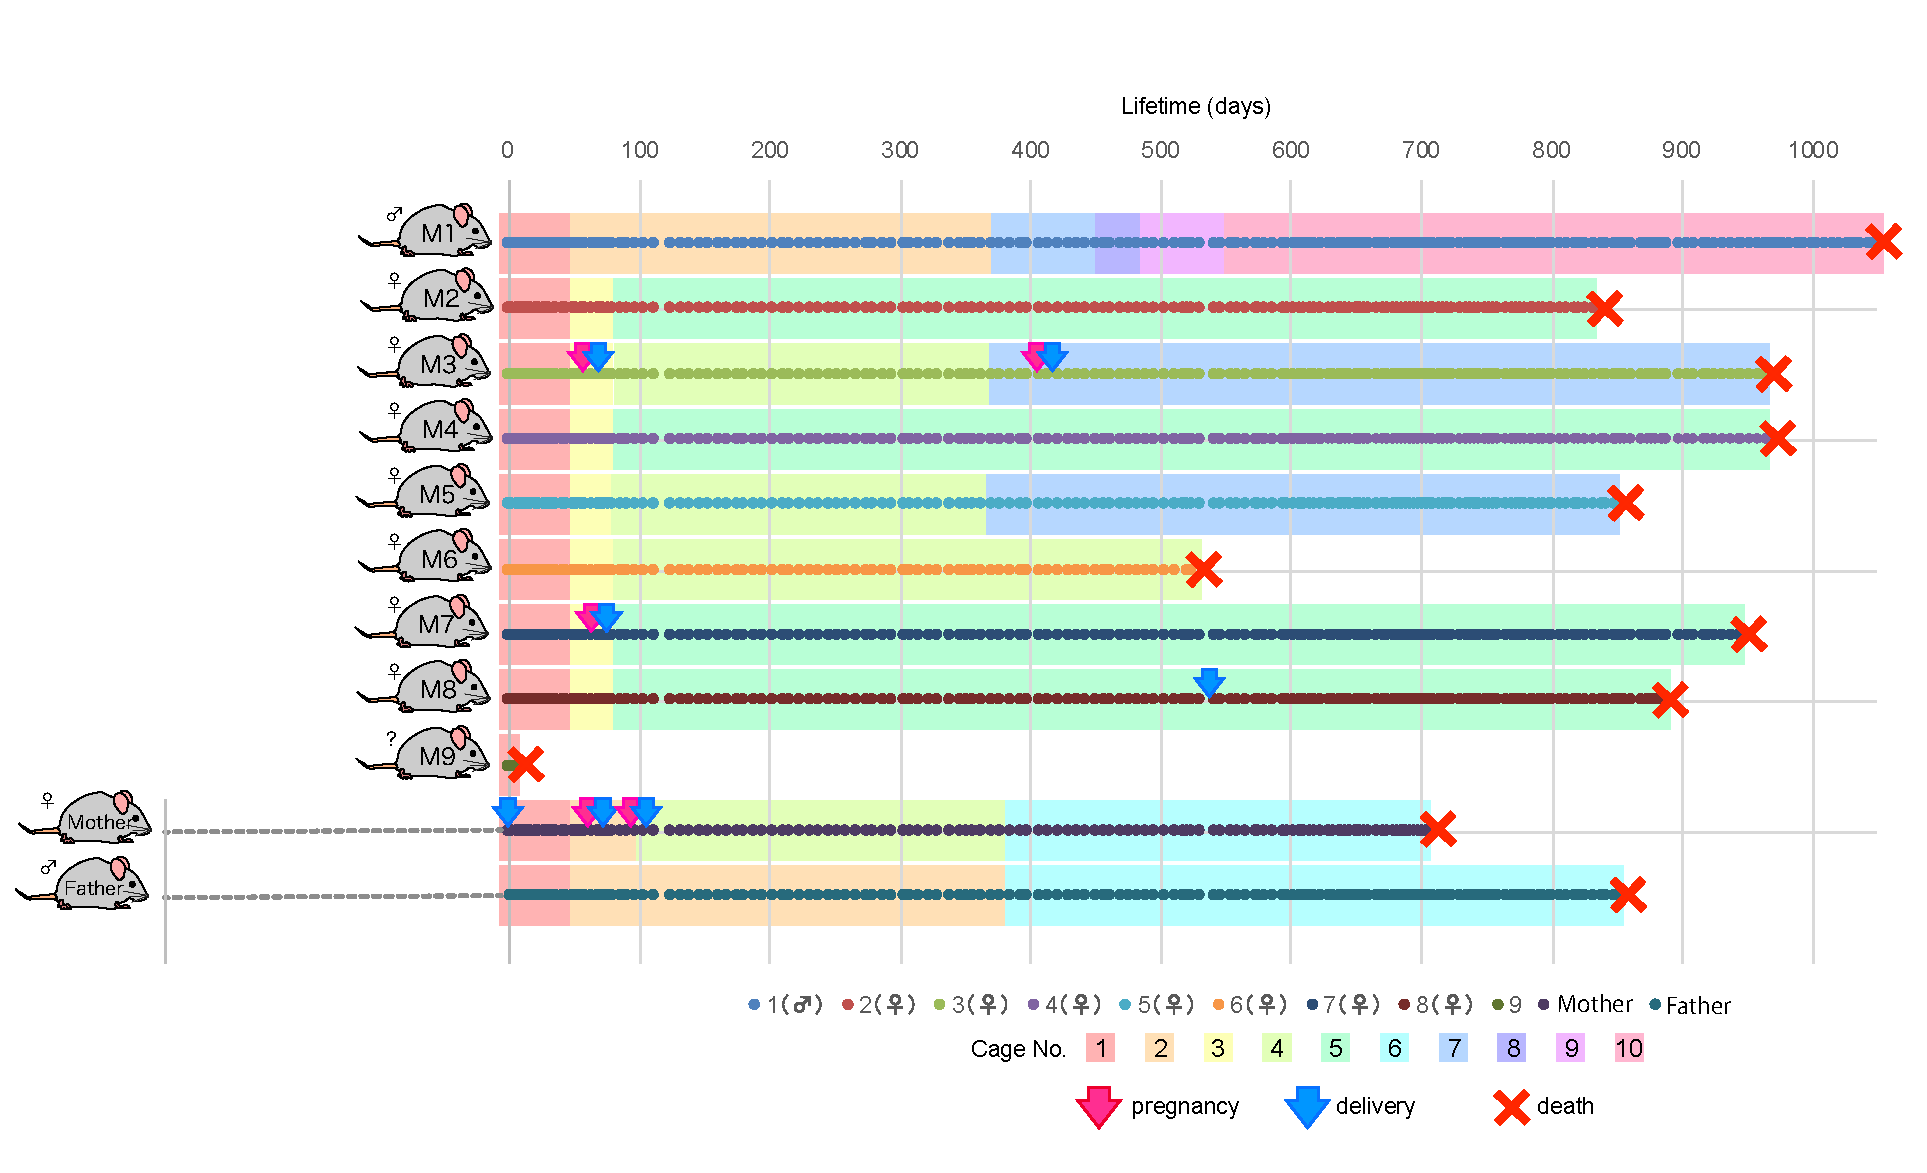
\includegraphics[width = 0.6\linewidth]{figures/chapter_2/fig_data.pdf}
}
\caption{}
\end{figure}

\newpage

\section{Summary Statistics}
\subsection{Rank- Abundance distributions}

\begin{figure}[H]
    \centering
    \includegraphics[width=\linewidth]{figures/chapter_2/RAD_mean.pdf}
    \caption{Caption}
    \label{fig:enter-label}
\end{figure}
\subsection{Sample composition across subjects}

\begin{figure}[H]
\centering
\subfigure[]{\includegraphics[width=0.48\linewidth]{figures/chapter_2/Phylum_stacked_first_100.pdf}}
\hfill
\subfigure[]{\includegraphics[width=0.48\linewidth]{figures/chapter_2/Class_stacked_first_100.pdf}}
\vspace*{1cm}
\subfigure[]{\includegraphics[width=0.48\linewidth]{figures/chapter_2/Order_stacked_first_100.pdf}}
\hfill
\subfigure[]{\includegraphics[width=0.48\linewidth]{figures/chapter_2/Family_stacked_first_100.pdf}}
\vspace*{1cm}
\caption{Caption}
\end{figure}

\begin{figure}[H]
    \centering
\includegraphics[width=0.9\linewidth]{figures/chapter_2/Genus_stacked_first_100.pdf}

    \label{fig:enter-label}
\end{figure}

\begin{figure}[H]\ContinuedFloat
    \centering
\includegraphics[width=0.9\linewidth]{figures/chapter_2/Species_stacked_first_20.pdf}
    \caption{Taxonomic ranks from bottom to top are:
Species $\subset$ Genus $\subset$ Family $\subset$ Order $\subset$ Class $\subset$ Phylum.}
    \label{fig:enter-label}
\end{figure}

\newpage
\section{Species abundance summary data \textcolor{red}{TO BE COMPLETED}.}
\input{tables/chapter_2/median_longtable}

As one can see by looking at the table \ref{tab:species_counts}, there are some species which are high in mean abundance while low in median abundance: these are species which are present during the first days of mice's lives and then drop rapidly to zero counts, meaning they go extinct or very rare. Some examples of such species are \textit{Streptococcus AY020}, \textit{Vibrio cholerae}, \textit{Eubacterium biforme}, \textit{Candidatus Arthromitus sp. SFB-mouse}, \textit{Streptococcus sp. B1} [Figure: \ref{fig:rare_species}]. In particular, some strains of \textit{Vibrio cholerae} are pathogenic and responsible for cholera disease. The data shows in that this bacterium is initially present in neonatal mice and then gets suppressed.  "Candidatus Arthromitus" sp. strain SFB-mouse-NL (SFB, segmented filamentous bacteria) is a commensal bacterium necessary for inducing the postnatal maturation of homeostatic innate and adaptive immune responses in the mouse gut \parencite{candidatus_arthromitus}.

\begin{figure}[H]
    \centering
    \includegraphics[width=\linewidth]{tables/chapter_2/rare_mean_species.pdf}
    \caption{Caption}
    \label{fig:rare_species}
\end{figure}
\newpage
\section{Gallery of timeseries plots.}


